\chapter{Theoretical Framework}
Mining data in a network is not a new subject. In fact, many different approaches have been suggested. It this section, we present some of them as the foundation for our project. We begin by describing basic graph theory, later moving on to link prediction in bipartite graphs. Moreover, measurements of nodes are discussed, including similarity, centrality and prestige. An introduction to Support Vector Machines from the perspective of classifying different nodes in a graph is given and lastly the concept of precision and recall along with cross-validation is presented.

\section{Graphs Representation}
\newcommand{\graph}{\textbf{G}}
\newcommand{\vertices}{\textbf{V}}
\newcommand{\edges}{\textbf{E}}
\newcommand{\weights}{\textbf{W}}
\newcommand{\adjmat}{\textbf{A}}

A graph $\graph=(\vertices,\edges)$ is defined as a set of vertices $\vertices$ of nodes and a set of edges $\edges$ connecting the vertices. A graph $\graph$ can be either undirected or directed, meaning that the edges in the graph has a direction or not. If there are multiple edges between a pair of vertices, the graph $\graph$ is denoted a multigraph.

One example of a graph is the internet, where each physical end device such as servers, computer and mobile phones are represented as vertices and the cables (or radio waves) connecting them are represented by edges. Another example is a social network with people as vertices and relationships between the individuals are the edges.

To each edge $e\in\edges$ there can be an assigned weight $w$. The weight can represent the strength of a relationship or a distance between vertices. Then the graph representation becomes $\graph=(\vertices,\edges,\weights)$

\subsection{The Adjacency Matrix}
Graphs can be represented in more than one way mathematically. One convenient way that allows for simple analysis is to represent a graph by its adjacency matrix $\adjmat$. Every Vertices $v\in\vertices$ is given an index $i \in [0,..,V]$ where $V = |\vertices|$. The element $a_{i,j}$ in $\adjmat$ is 1 if the graph $\graph$ contains an edge from vertices $i$ to vertices $j$ if the graph is undirected $a_{i,j}=a_{j,i}\, \forall i,j$\cite{adj_matrix}. If the graph is weighted then $a_{i,j} = w(i,j)$. Furthermore, if the graph is a multigraph, the adjacency matrix becomes 3 dimensional, where each layer in the third dimension represents a different kind of relation between vertices.

\subsection{Graph metrics}
In this section we will introduce some common attributes definitions of graphs, global (attributes on the graph itself) and local (attributes of nodes or edges).

The order of the graph is defined as the number of vertices $V=|\vertices|$, and the size is defined as the number of edges $E=|\edges|$. The distance $d(u,v)$ between to vertices $u\in\vertices$ and $v\in\vertices$ is the smallest number of edges needed to connect $u$ and $v$. The eccentricity $\epsilon(v)$ of a vertex is the greatest distance to any other vertex in the graph. The diameter of the graph $\graph$ is the greatest distance between any pair of node\cite{graph_theory}, 
$$d(\textbf{G}) = \max_{v \in V}\epsilon(v)$$

A global measurement for how well the vertices in the graph is connected and how sparse the adjacency matrix is, can be measured be the density of the graph. For undirected graphs it is defined as\cite{density}
$$D =  \frac{2|E|}{|V|\,(|V|-1)}.$$
For directed graphs it is
$$D = \frac{|E|}{|V|\,(|V|-1)}.$$

\subsection{The Bipartite Graph}\label{subsec:bigraph}
A special kind of graph is the bipartite graph where the vertices can be divided into two adjacent sets and where every edge has one end in each of the two adjacent sets. This kind of graph is common in social networks. An example is where one of the sets is a buyer class and the other set is a product class. Such graph may stem from a web shop or a movie streaming service. Since the bipartite graph is a special case of the general graph \graph, the same metrics and methods can be used, but in many cases they can be simplified. The adjacency matrix of the bipartite graph can be simplified since edges within any of the two sets are by the definition forbidden. Furthermore, since the direction of the edge is given implicitly by the natural structure of the graph, for example a product does not buy a buyer but the other way around the bipartite graph can be considered undirected. This lets us define the adjacency matrix of a bipartite graph by letting the rows represent one of the two sets and the columns the other set. By this construction all information about the graph is contained in the adjacency matrix. This means that the size of the adjacency matrix is only 1/4 of the adjacency matrix of the general graph. The relationship between the bipartite adjacency matrix $\textbf{W}$ and the adjacency matrix $\adjmat$ is
$$
\textbf{A} = \left[
\begin{matrix}
  \textbf{O}_x & \textbf{W} \\
  \textbf{W}^T & \textbf{O}_y
\end{matrix}
\right]
$$
Where $\textbf{0}_x$ and $\textbf{0}_y$ only contain zeros due to the definition of the bipartite graph that all edges has one endpoint in each of the two sets. Due to the undirect nature of the bipartite graph, the bottom left part of $\adjmat$ equals the transpose of the upper right part which we take as the adjacency graph for the bipartite graph.

Note that since the size of the two adjacent sets are not generally the same, $\textbf{W}$ is not square in the general case and not symmetric unlike $\adjmat$ in the general case of undirected graphs.

By using $\textbf{W}$ we can define the density D for the bipartite graph simply as 
$$\text{D} = \frac{\sum_{i,j}e_{i,j}}{|\textbf{W}|}
$$
where $i,j$ run over all rows and columns in $\textbf{W}$ and
$$e_{i,j} =
    \left\{
        \begin{matrix}
            1\quad \text{if $w(i,j)\, >\, 0$} \\
            0\quad \text{otherwise}
        \end{matrix}
    \right. ,
$$
in other words, the number of edges in the graph divided by the number of possible so that D = 0 if there are no edges and D = 1 if all possible edges exists in the graph. We will return to the bipartite graph in the next chapter.


\section{Link Prediction in Bipartite Graphs}
The recent year's growth of large social networks, such as those from large consumer sites as Amazon and social sites as Facebook and LinkedIn, have yielded an increasing interest in network analysis. But a network graph might only disclose a part of a large picture or might change over time, therefore it is useful to develop methods for link prediction.

The aim of link prediction analysis is to predict future edges in a temporal graph or discover hidden links in a graph by considering the topological structure of the graph. Many recent approaches that aim at predicting edges in social networks are similarity based, where a vertex pair index is used to indicate the similarity of the two nodes. The index value is used to make predictions about the likelihood of future links. There are many different attributes that can be used to indicate similarity. The similarity index can be global, local or quasi-local. The methods that are local only consider the information about the closest neighborhood. Example of methods that are local are Common Neighbors, Jaccard index, Hub Promoted and Resource Allocation \cite{linkpredict}. The global methods use topological information about the whole graph and include Katz, and Matrix Forest Index \cite{linkpredict}. The quasi-local methods do not require information about the whole graph but requires more information than the local ones. Another type of similarity method is random walk methods including SimRank, Cos+ and Average Commute Time \cite{linkpredict}. There has also been a lot of work where Machine Learning strategies have been used for link prediction \cite{mlpredict1,mlpredict2,mlpredict3,mlpredict4,mlpredict5,mlpredict6,mlpredict7}.

\subsection{Projection-based Link Prediction}\label{sec:plp}
In this chapter a very recently developed algorithm by \citet{plp} for link prediction in bipartite graphs is presented. The algorithm utilizes a concept the authors call candidate node pair CNP wich lets the algorithm disregard a large part of the network. This reduces the running time to $O(m)$ where $m$ is the size of the smallest of the two adjacent sets of the bipartite graph.

As an introduction to the algorithm, the intuitive idea behind the algorithm is to predict links between pairs of vertices in the bipartite graph that do not have the effect of creating new secondary relations between two vertices in the same set. This is done by looking at similarities between vertices and their connections and giving a higher probability if the similarities between vertices is of a unique kind, meaning that the similarity is not shared by others. An example of an bipartite graph of attackers $U$ and targets $V$ is shown in \figref{fig:cnp}. A more detailed description follows.

\paragraph{Projected Graph}
A bipartite graph $\textbf{G} = (\textbf{U},\textbf{V},\textbf{E})$ can be projected onto a unipartite graph $\textbf{G}_u = (\textbf{U},\textbf{E}_u)$ where all vertices belong to $\textbf{U}$ and two vertices $A,B\in\textbf{G}_u$ are connected by an edge $e\in\textbf{E}_u$ if both have at least one common neighbor in $\textbf{V}$. We call this the U-projected graph. In a similar fashion $\textbf{G}_v = (\textbf{V},\textbf{E}_v)$ is the V-projection graph. The U-projection and V-projection of the bipartite graph in \figref{fig:cnp} is shown in \figref{fig:plp_u} and \figref{fig:plp_v} respectively.

\paragraph{Candidate Node Pairs}
A candidate node pair CNP by U-projection is a pair of nodes $(B,l)$ with $B\in\textbf{U}$ and $l\in\textbf{V}$ such that $(B,l)\notin\textbf{E}$ and $\textbf{G}_u=\textbf{G}'_u$ where $\textbf{G}'_u$ is the U-projection of $\textbf{G}'=(\textbf{U},\textbf{V},\textbf{E}\cup\{(B,l)\})$.

In other words, a CNP by U-projection is a pair of vertices that we can add a new edge between in the bipartite graph $\textbf{G}$ without changing the U-projection. 

It can be shown \cite{plp} by the theorem of CNP symmetry that  a node pair $(B,l)$ is CNP by V-projection if and only if a $(B,l)$ is a CNP by U-projection. This is important since it lets us do the computations on the smallest of the two sets $\textbf{U}$ and $\textbf{V}$ only.

It can also be shown \cite{plp} that a node pair $(B,l)$ is a CNP if and only if 
$$
\mathbf{\Gamma}_{u,B}\cap\bm{\Gamma}_l \neq \varnothing\text{ and } B\notin \mathbf{\Gamma}_l.
$$
where $\bm{\Gamma}_{u,B}$ is the set of nearest neighbors of B in the u-projection and $\bm{\Gamma}_l$ is the set of nearest neighbors of l in the bipartite graph. Namely there must be at least one vertex $C\in\textbf{U}$ with $(C,x)\in\textbf{E}$ and also $(C,B)\in\textbf{E}_u$, otherwise the U-projection of $\textbf{G}'\neq\textbf{G}$. By the theorem of CNP symmetry the same is true for $\bm{\Gamma}_{v,l}\cap\bm{\Gamma}_{B}$.

\paragraph{Patterns Covered by a CNP}
A pair of vertices $A$ and $B$ in $\textbf{U}$ is called a pattern in $\textbf{G}$ if there exist a vertex $l\in\textbf{V}$ such that $(A,l),(B,l)\in\textbf{E}$. With $(B,l)$ a CNP in $\textbf{G}$ for each vertex $C\in\bm{\Gamma}_{u,B}\cap\bm{\Gamma}_{l}$ we call $\{B,C\}$ in $\textbf{G}$ a pattern covered by the CNP $(B,l)$.

A CNP can cover more than one pattern. The more patterns a CNP covers the greater the likelihood that the CNP becomes an edge in the future because a pattern covered by a CNP indicates that a similar edge already exist. As an example, consider the case in \figref{fig:cnp} were $\textbf{G}$ represents an attack graph with $\textbf{U}$ being the set of all attackers and $\textbf{V}$ the set of all targets. Consider the CNP ($U_2$,$V_3$) where $U_2$ attacks target $V_3$. The patterns $\{U_2,U_1\},\{U_2,V_4\}$ covered by ($U_2$,$V_3$), all already exist due to the connections through $V_1$ and $V_4$ respectively, which indicates that the probability of $U_2$ attacking $V_2$ is high.

On the other hand, for a pair of vertices $(B,l)$ that is not a $C\in\bm{\Gamma}_{u,B}\cap\bm{\Gamma}_{l} = \varnothing$ and hence we can not find a similar pattern for pair $(B,l)$ which means that the future existence of the edge $(B,l)$ is unlikely. This is key for the running time being $O(m)$ since we only have to compute a predictive index for the pair of vertices that are CNP.

\paragraph{The Connectivity of a CNP}
By the definition of Patterns Covered by a CNP the number of patterns covered by a CNP $(B,l)$ is $|\bm{\Gamma}_{u,B}\cap\bm{\Gamma}_{l}|$, with $|\cdot|$ being the set size. As shown by the example above, this is a good measurement for the likelihood of the link $(B,l)$ being in existence in the future.

\begin{figure}[!ht]
\centering
\input{images/cnp_example.pdf_t}
\caption{The bipartite graph representation $\textbf{G}=(\textbf{U},\textbf{V},\textbf{E})$ of attackers $U_i\in\textbf{U}$ and targets $V_j\in\textbf{V}$. The dashed line represents the CNP ($U_2,V_3$).\label{fig:cnp} }
~
\\[0.5cm]
\input{images/plp_example_u.pdf_t}
\caption{U-projection unipartite graph  $\textbf{G}_u=(\textbf{U},\textbf{E}_u)$ of the bipartite graph in \figref{fig:cnp}. Notice how the the potential edge $(U_2,V_3)$ represented by the dashed line in \figref{fig:cnp} would not change the U-projection since, that edge would imply edges $(U_2,U_1)$ and $(U_2,U_4)$ but as we can see they already exist in the U-projection.\label{fig:plp_u}}
~
\\[0.5cm]
\input{images/plp_example_v.pdf_t}
\caption{V-projection unipartite graph $\textbf{G}_v=(\textbf{U},\textbf{E}_v)$ of the bipartite graph in \figref{fig:cnp}.  Notice how the the potential edge $(U_2,V_3)$ represented by the dashed line in \figref{fig:cnp} would not change the V-projection since, that edge would imply edges $(V_3,V_1)$, $(V_3,V_2)$ and $(V_3,V_4)$ but as we can see they already exist in the V-projection.\label{fig:plp_v}}
\end{figure}

\paragraph{Pattern Weights}
When using the numbers of patterns covered by a CNP as the likelihood of future edges, some useful topological information about the bipartite graph $\textbf{G}$ is lost. This is solved by adding weights to the corresponding edges in the U-projection. The weight of $(A,B)\in\textbf{E}_u$, $w_u(A,B)$ is computed using three different topological features:
\begin{enumerate}
\item The numbers of common neighbors of nodes $A$ and $B$, $|\bm{\Gamma}_{A}\cap\bm{\Gamma}_{B}|$.
\item The degrees of the common neighbors of $A$ and $B$.
\item The degree of $A$ and $B$.
\end{enumerate}
A pattern ${A,B}$ in $\textbf{G}$ is represented by an edge $(A,B)$ in $\textbf{G}_u$ which tells us that $A$ and $B$ have a common neighbor in $\textbf{G}$, however since the topological information about how many such common neighbors $A$ and $B$ have is lost in the projection, we want the weight $w_u(A,B)$ to contain that information. If a common neighbor $x\in\textbf{V}$ of $A$ and $B$ have a large degree it makes the path between $A$ and $B$ through $x$ further away from unique and therefore less significant and therefore the weight should be reduced. The same reasoning goes for the degree of $A$ and $B$ itself and we end up with the weight of pattern $\{A,B\}$ (and the weight of edge $(A,B)\in\textbf{E}_e$)
$$
    w(A,B) = \frac{2}{|\bm{\Gamma}_{A}|+|\bm{\Gamma}_{B}|} \sum_{x\in\bm{\Gamma}_{A}\cap\bm{\Gamma}_{B}} \frac{1}{|\bm{\Gamma}_{x}|}
$$

\paragraph{Predictive Index of a CNP}
With the topological information preserved in the edge weights of the U-projected graph we are ready for the definition of the predictive index of a candidate node pair
$$
 c(B,l) = \sum_{C\in\bm{\Gamma}_{u,B} \cap \bm{\Gamma}_{l} } w(B,C)
$$
The index is the summation of weights of corresponding patterns covered by $(B,l)$. We know that the more patterns with large weights a CNP covers the greater the likelihood of a future edge $(B,l)$ and therefore this is the value used for future link prediction.

The description of the algorithm can be found in Appendix \ref{ap:plp} and the complexity analysis done by the original authors in \cite{plp}.


\section{Similarities Between Nodes \label{sim}}
Quantifying the similarities between vertexes in a network can be of great interest. In many situations it is useful to be able to determine what other nodes are similar to a specific node. However, two nodes can be similar in many different ways. For instance, they may have the same degree, the same neighbour, or be a part of the same community. Thus, there are numerous approaches to take when defining similarity measures.

Two vertexes are said to be structurally equivalent if they share many neighbors \cite{leicht2006}. Taken in a social network perspective, it seems reasonable to think that two persons have something in common of they have many common friends. Below we present some similarity measures based on structural equivalence.

\subsection{Local similarity}
Local similarity measures exploit the local structures of an undirected graph $G$ \cite{fouss2016algorithms}. Let $\bm{\Gamma}_i$ be the neighborhood of node $i$ in a network. The common friends of node $i$ and $j$ are thus given by
\begin{equation}
\label{common}
\sigma_{common} = |\bm{\Gamma}_i \cap \bm{\Gamma}_j| = \sum_{k=1}^n a_{ik}a_{kj}
\end{equation}
%where $|x|$ refers to the cardinality of the set $x$ such that $|\bm{\Gamma}_x |$ gives the degree of node $x$. 
The expression above is the basis of the following similarity measures that will be presented. The expressions will be presented both from the notation of neighbours $\bm{\Gamma}$ and also the adjacency matrix $\textbf{A}$.

\textbf{Cosine coefficient.} In an undirected graph, the cosine coefficient is simply the normalization of the score of common neighbors of node $i$ and $j$ \cite{fouss2016algorithms}
\begin{equation}
    \label{cosine}
    \sigma_{cosine} = \frac{|\bm{\Gamma}_i \cap \bm{\Gamma}_j|}{\sqrt{|\bm{\Gamma}_i||\bm{\Gamma}_j|}} = \frac{\sum_{k=1}^n a_{ik}a_{kj}}{\sqrt{a_{i \circ }a_{\circ j}}}
\end{equation}
$a_{i \circ }$ denotes the summation of row $i$ in the adjacency matrix while $a_{\circ j}$ denoted the column $j$ of the adjacency matrix.

Generally speaking, the cosine coefficient between two node vectors $\textbf{v}_i$ and $\textbf{v}_j$ defined by $\textbf{v}_i^T\textbf{v}_i/(\|\textbf{v}_i\|\|\textbf{v}_j\|)$ is a measure of the linear relationship between the two node vectors. Thus, the nodes are considered more similar the smaller the angle between the node vectors in the node space is.

\textbf{Jaccard index.} The Jaccard index is computed as follows
\begin{equation}
    \label{jaccard}
    \sigma_{Jaccard} = \frac{|\bm{\Gamma}_i \cap \bm{\Gamma}_j|}{|\bm{\Gamma}_i \cup \bm{\Gamma}_j|} = \frac{\sum_{k=1}^n a_{ik}a_{kj}}{a_{i \circ }+a_{\circ j}-\sum_{k=1}^n a_{ik}a_{kj}}
\end{equation}
The denominator represents the number of neighbors belonging to at least one of the two nodes $i$ or $j$. Thus, the Jaccard index is the fraction of common neighbors in relation to the cardinality of the union of neighbors. 

\textbf{Dice coefficient.} The Dice coefficient is defined accordingly
\begin{equation}
    \label{dice}
    \sigma_{Dice} = \frac{2 |\bm{\Gamma}_i \cap \bm{\Gamma}_j|}{|\bm{\Gamma}_i|+|\bm{\Gamma}_j|}= \frac{2\sum_{k=1}^n a_{ik}a_{kj}}{a_{i \circ }+a_{\circ j}}
\end{equation}
Defined in words, the Dice coefficient is calculated as twice the number of common neighbors divided by the sum of the cardinalities of the two neighborhoods. 

\textbf{Hub-promoted index.} The index promotes hubs in the network and is given by
\begin{equation}
    \label{prohub}
    \sigma_{prohub} = \frac{|\bm{\Gamma}_i \cap \bm{\Gamma}_j|}{\min(|\bm{\Gamma}_i|,|\bm{\Gamma}_j|)} = \frac{\sum_{k=1}^n a_{ik}a_{kj}}{\min(a_{i \circ },a_{\circ j})}
\end{equation}
Since the denominator is based on the lower degree only, the links adjacent to hubs are likely to be assigned high scores \citep{lu2011}. The measure is also called overlap similarity \citep{fouss2016algorithms} since a perfect score of 1 implies that the neighborhood of one of the nodes is a subset of the neighborhood of the other node.

\textbf{Hub-depressed index.} The hub-depressed index depresses hubs in the network \citep{fouss2016algorithms}
\begin{equation}
    \label{dehub}
    \sigma_{dehub} = \frac{|\bm{\Gamma}_i \cap \bm{\Gamma}_j|}{\max(|\bm{\Gamma}_i|,|\bm{\Gamma}_j|)} = \frac{\sum_{k=1}^n a_{ik}a_{kj}}{\max(a_{i \circ },a_{\circ j})}
\end{equation}
In contrast to the denominator in the hub-promoted index, this denominator takes the higher degree into consideration. Thus, links adjacent to hubs are likely to be assigned low scores. 

\begin{comment}
\textbf{Adamic index.} 
\begin{equation}
    \label{adamic}
    \sigma_{Adamic} = \frac{|\bm{\Gamma}_i \cap \bm{\Gamma}_j|}{\log(|\bm{\Gamma}_i|,|\bm{\Gamma}_j|)} = \frac{\sum_{k=1}^n a_{ik}a_{kj}}{\max(a_{i \circ },a_{\circ j})}
\end{equation}
\end{comment}

\subsection{Global similarity}
A global similarity measure takes the topology of the whole graph into account. Comparing with the local indices, the global ones can give more accurate predictions \citep{lu2011}.

\textbf{Katz Index.} One global index is the Katz index, defined below \citep{fouss2016algorithms}.
\begin{equation}
    \textbf{K}_{Katz}=\sum_{t=1}^{\infty} \alpha^t \textbf{A}^t = (\textbf{I}-\alpha \textbf{A})^{-1}-\textbf{I}
\end{equation}
The parameter $\alpha \in [0,1]$ defines an attenuation factor to discount the importance of common neighbors far away. In other words, $\alpha$ determines how much the similarity should be dependent om common neighbours far away.

The accuracy of a global index is given at the expense of complexity. Since the global indices take the topology of the whole network into account, the measures can be very time-consuming to compute and thus inappropriate for large-scale networks. 

\subsection{Quasi-local similarity}
There is a tradeoff called quasi-local indices. As the name indicates, they are based on more information than the local indices but eliminate nodes too far away in the network. According to \citet{lu2011}, the result is less time consuming algorithms with higher accuracy than the local indices, since superfluous information, contributing with little improvement in accuracy, is ignored.

\textbf{Local Path Index} The Local Path (LP) Index is a quasi-local similarity index which provides a good tradeoff between the accuracy and computational complexity \citep{lu2011}. It is defined as 
\begin{equation}
    \label{lp}
    \sigma_{LP} = \textbf{A}^2+\alpha \textbf{A}^3
\end{equation}
where $\textbf{A}$ denotes the adjacency matrix of the graph. Taking the square of the adjacency matrix gives the number of paths there is between node $i$ and node $j$ with length 2. Moreover, $\textbf{A}^3$ given the number of paths between two nodes with length 3. 

$\alpha$ is a discounting factor which relates to the importance of having the same neighbour two steps away. Thus, a high value of 1 indicates high importance, making a common neighbor two steps away as important as having a common nearest neighbor. Setting $\alpha$ to 0 degenerates the expression to only account for the nearest neighbors, thus making the Local Path Index equal to $\sigma_{common}$, see equation \eqref{common}.

\section{Centrality}
By exploiting the structure of a graph or a subgraph, the \textit{centrality} of a node can be determined. 

Centrality is a measure that is calculated on undirected graphs. Dealing with directed graphs, these similarity measures are instead called \textit{prestige} or \textit{importance} measures. \cite{fouss2016algorithms}


\subsection{Closeness Centrality}
The closeness centrality measure indicates the proximity of a node $i$ to a node $j$ in an undirected graph $G$. The measure implies to what extent node $i$ is central to $G$, hence, how representative it is to the network \citep{fouss2016algorithms}. The node with the highest centrality score is the most central node.

According to \citet{fouss2016algorithms}, the most popular choice for quantifying the closeness centrality is
\begin{equation}
    cc_i=\frac{1}{\sum_{j=1}^{n} \Delta_{ij}}
\end{equation}
where $\Delta_{ij}$ denotes the shortest-path distance between the nodes $i$ and $j$, and $n$ is the number of nodes in the graph. The most central node is the one closest to all the rest of the nodes. For the case with an unweighted, undirected graph, the highest closeness centrality is found for a node adjacent to all the rest. The closeness centrality is then given by $\frac{1}{n-1}$.

\subsection{Betweenness Centrality}
Betweenness centrality can be used to quantify to what extent a node is an important intermediary \citep{fouss2016algorithms}. Nodes with high betweenness are very important since many of the other nodes communicate through them \citep{Kajdanowicz2013}. 

The best-known walk based centrality measure is Freeman's betweenness centrality \citep{fouss2016algorithms}. It is also known as the shortest-path betweenness centrality and is computed by taking the shortest paths $p_{ik}^*$ going through an intermediate node $j$, where $i\neq j \neq k\neq i$ for all the node pairs $i$ and $k$. The shortest path between node $i$ and $k$ as $p_{ik}^*$ is then a subset of all the shortest paths denoted as $P_{ik}^*$ connecting node $i$ and $k$. Thus, the number of shortest paths between the two nodes are given by $|P_{ik}^*|$. Moreover, we denote the total number of shortest paths between node $i$ and $k$ going through node $j$ as $\eta(j \in P_{ik}^*)$. In accordance with the notation used in \citep{fouss2016algorithms} we can now formulate the shortest-path betweenness centrality as follows
\begin{equation}
    \text{bet}_j=\sum_{i=1, i\neq j}^{n} \sum_{k=1, k \neq i,j}^{n} \frac{\eta(j \in P_{ik}^*)}{|P_{ik}^*|}
\end{equation}
A more intuitive way of putting it is that the betweenness centrality measures how many times node $j$ is on the shortest path between two nodes in the graph. Hence, it gives an indication of important the node is for the communication of a network. 

\section{Prestige}
Prestige or importance measures are very similar to the concept of centrality but differs in the sense that it is applied on directed graphs instead of undirected graphs. 

\subsection{PageRank}
The PageRank algorithm was developed in 1998 in order to rank web pages and is one of the algorithms Google currently uses in the Google search engine \cite{langville2004deeperinside,langville2012}. The PageRank score is based on the number of times a node is cited by other nodes, taking the node's importance into account. The PageRank algorithm assigns a prestige score to every node in the network. According to \citet{fouss2016algorithms}, the prestige score can in its most basic form be calulcated as 
\begin{equation}
    x_j=\sum_{i=1}^{n} \frac{a_{ij}x_i}{a_{i\circ}}
\end{equation}
where $x_i$ is the prestige score associated with a node $i$ and $a_{ij}$ is an element in the non-symmetric adjacency matrix $\textbf{A}$, and $a_{i\circ}$ denotes the outdegree of node $i$. 

As a result, a node $j$ receives a high PageRank score if it is related to many other nodes, if the nodes adjacent to $j$ have high prestige scores themselves and the neighbors to node $j$ have a small outdegree. 

% Difference between PageRank and HITS. Refer to langville2004; HITS is more costly

\section{Support Vector Machine \label{svmTheory}}
Support Vector Machines (SVM) is a set of supervised learning methods originally developed for binary classification \citep{Hsu2002}. SVMs work well in practice and have been applied to various fields, such as face identification, text categorization and bioinformatics \citep{campbell2011}. In this section, we will only briefly describe the theory behind SVM. For a more rigorous description, we refer to \citep{Kecman2005,Cortes1995,campbell2011}.

Let us consider some training data, composed by the input vectors $\bm{x}_i\in \mathds{R}^p$ where $i=1,...,n$ and and $n$ denotes the number of classified samples. Every input vector is related to a target $y_i \in \{-1,1\}$. The training data can be viewed as labelled data in an input space. The learning task is finding a directed hyperplane that maximizes the distance from the two classes of labeled datapoints. A graphical representation of a hyperplane can be found in figure \ref{svm}. 

\begin{figure}[h!]
    \centering
    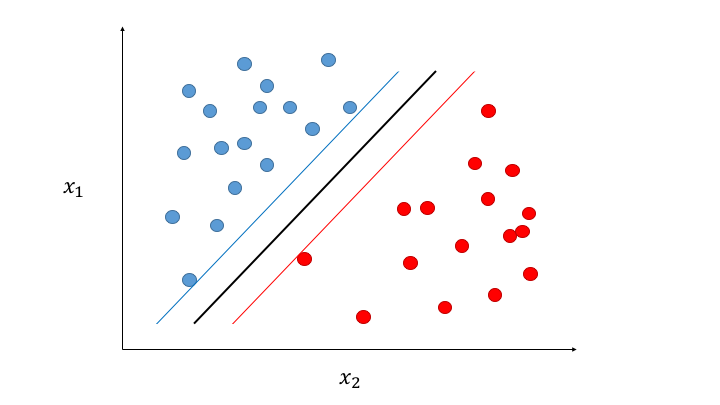
\includegraphics[width=0.75\textwidth]{svm.png}
    \caption{The feature space of a binary data set. The black line illustrates the optimal hyperplane, dividing the two classes. Two \textit{hard} boundaries are represented as the blue and red lines. The optimal hyperplane is found when the distance between the three lines are maximized.}
    \label{svm}
\end{figure}

The optimal hyperplane is given by \citep{campbell2011}
\begin{equation}
    \bm{w}\cdot\bm{x}+b=0
\end{equation}
where $\bm{w}$ is are the weights, perpendicular to the hyperplane, and $b$ denotes the bias or offset which displaces the hyperplane from the origin. This is found by maximizing the margins between the closest samples and the hyperplane, which according to \citet{campbell2011} can be defined as minimizing $$\frac{1}{2}||\bm{w}||_2^2=\frac{1}{2}\bm{w}\cdot\bm{w}$$

In the example given in figure \ref{svm}, we presented a simple task where the two classes are linearly separable. In reality, it may be much more complicated and clusters could be highly intermeshed \citep{campbell2011}. Thus we now introduce the function $\phi(\cdot)$, which defines the mapping from input space to feature space with higher dimensionality. Moreover, many real life datasets contain noise and outliers, leading to poor generalisation. A way of handling this is to introduce a slack variable $\xi_i$, which imposes a relaxation of the hard boundaries. The boundary then becomes a soft margin where in addition to maximizing the margin, we want to minimize the sum of errors $\sum \xi_i$. Applying the method of Lagrange multipliers, \citet{campbell2011} formalize SVM to the following problem
\begin{align}
    \nonumber
    \min_{\bm{w},b,\bm{\xi}}\text{~~}&\frac{1}{2}\bm{w} \cdot \bm{w}+C\sum_{i=1}^{n} \xi_i \\ 
    \text{subject to~~}&y_i(\bm{w}\cdot \phi(\bm{x}_i)+b)\geq 1-\xi_i \label{svmeq}\\ 
    &\xi_i\geq 0 \nonumber
\end{align}
where $C>0$ is the penalty parameter for the error term. Solving this problem will find a hyperplane to set the decision boundary in the high dimensional space $\phi$.

A central concept in SVM is the kernel. The kernel function relates to the mapping function $\phi$ and is given by $K(x_i,x_j)=\phi(x_i)\cdot \phi(x_j)$. Three common kernels are the linear kernel, the polynomial kernel, and the Radial Basis Function (RBF) kernel presented in the same order below
\begin{align}
K(\bm{x}_i,\bm{x}_j)&=\bm{x}_i \cdot \bm{x}_j & \nonumber \\ 
K(\bm{x}_i,\bm{x}_j)&=(\gamma \bm{x}_i \cdot \bm{x}_j + r)^d \text{~~~~~}&\gamma>0\\
K(\bm{x}_i,\bm{x}_j)&=exp(-\gamma ||\bm{x}_i-\bm{x}_j||^2) \text{~~~~~}&\gamma>0 \nonumber
\end{align}
The kernel and its parameters ($\gamma$, $r$ and $d$) are highly dependent on the task itself and have to be properly chosen. Although it may be very costly, one way of choosing parameters is to perform grid search in combination with cross-validation \citep{Hsu10apractical}.

To conclude, the SVM maps the input vectors to a high dimensional feature space, where a decision surface is constructed. One property of the SVM classifier is that it minimizes the empirical classification error as well as maximizes the geometrical space between the samples and the constructed hyperplane \citep{Cortes1995}.

\subsection{One-against-one}
Much research has been devoted towards multi-class SVM. \citet{Hsu2002} have made a comparison of the one-against-all, one-against-one and Directed Acyclic Graph Support Vector Machines (DAGSVM) methods. In their paper, \citet{Hsu2002} conclude that one of the more suitable methods for practical use is the one-agains-one. One-against-one constructs one SVM for each pair of classes. Hence, a problem with $c$ classes would impose $c(c-1)/2$ binary SVMs, each trained on data from only two classes.

\subsection{Unbalanced data \label{unbalanced}}
Since the SVM divides classes by finding the hyperplane that maximizes the margin, it imposes a problem with unbalanced data. A problem with unbalanced data arises when there is a notable difference between the number of samples in different classes \cite{delRio2014}. The class containing the fewest number of samples is referred to as the minority class while the class with the highest number of samples is referred to as the majority class. The imbalance of datapoints will shift the hyperplane towards the marginal class, resulting in a bias towards the majority class and a low performance towards the minority class. See figure \ref{unbalancedSVM} for an illustration of the issue of unbalanced datasets, where the learned hyperplane does not coincide with the ideal one. 

\begin{figure}[h!]
    \centering
    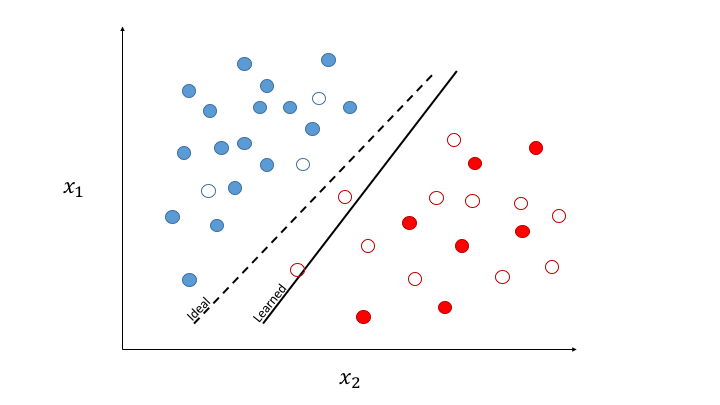
\includegraphics[width=0.75\textwidth]{svmImbalanced.png}
    \caption{Illustration of the problem with unbalanced data. The learned hyperplane does not coincide with the ideal one implicating bad classifications. The filled circled belong to the training set. The empty circles represent datapoints in the population that is not included in the training set.}
    \label{unbalancedSVM}
\end{figure}

In some cases unbalanced data becomes a big problem. \citet{delRio2014} mention the presence of this problem in real-world applications such as finance, software defect detection and medical diagnosis. One example where this issue arises is the identification of cancer patients among people. The majority of the people are not sick with cancer, however, it is more crucial to classify the cancer patients correctly than it is to classify the healthy people correctly. 

To deal with unbalanced data, different approached can be taken. It is possible to address the issue by constructing a dataset with a uniform distribution, either by performing undersampling or oversampling \citep{delRio2014}. Undersampling methods simply undersamples the majority class, i.e. the class with many data. However, this could lead to the issue of ending up with a small dataset and might not be the best choice for SVM \citep{Akbani2004}. 

Oversampling methods oversamples the minority class, such that new instances of data belonging to the minority class is created \citep{delRio2014,Akbani2004}. The number of datapoints in each class will then equal the number of datapoints in the majority class present in the unbalanced dataset. There are many different algorithms, with varying performance, for performing oversampling. The methods can be complex and the performance is dependent on the task. However, there is another way of dealing with unbalanced datasets in SVM, namely to weight the classes. Class weights are easily implemented and has been shown to offset the effect of unbalanced data \citep{Akbani2004}. The weight is then a factor to the penalty term, given in equation \eqref{svmeq}.

The above example with cancer patients also serves as a good illustration of the issue of receiving good accuracy in an unbalanced dataset. Imagine only 2\% of the people have cancer, if the classifier classifies all people as non-cancer patients, an accuracy of 98\% will be reached. This seems to be a good accuracy however, none of the cancer patients will be identified. Thus, the seemingly good classifier will therefore be useless for its purpose. Hence, when dealing with unbalanced datasets, it is preferable to segment the accuracy of each class \citep{delRio2014}. 

\subsection{Scaling \label{scale}}
\citet{Hsu10apractical} address the issue of varying magnitudes of the attributes in $\bm{x}_i$. To avoid that attributes of higher order of magnitude dominate other attributes, all features should be scaled. As a result, another advantage arises since scaling the values can avoid numerical difficulties. \citet{Hsu10apractical} recommend to normalize the values to the range [-1,1] or [0,1].

\section{Precision and Recall}
To evaluate the performance of a binary classifier, the concepts of precision and recall are useful. Precision measures the retrieved instances that are relevant while recall measures how many of the relevant instances that are retrieved. Another way of putting it is to say that precision is a measure of confidence while recall gives the sensitivity \citep{powers2011}.

The measurements are calculated from the number of True Positives (TP), False Positives (FP) and False Negative (FN). Precision and recall are calculated by \citep{powers2011}
\begin{align}
\text{Precision}&=\frac{TP}{TP+FP}\\
\text{Recall}&=\frac{TP}{TP+FN}
\end{align}
To be exhaustive in the notation, there is also the case of True Negative (TN) although it is never used in the computation.

To evaluate binary classifiers, the Area Under Curve (AUC) can be calculated. AUC$\in[0,1]$ where a high value reflects a good classifier. The AUC is simply calculated as the integral of the prediction-recall curve.

Furthermore, there is the F$_1$ score reflecting the classifiers accuracy. The F$_1$ score is calculated as the harmonic mean of precision and recall \citep{powers2011}
\begin{equation}
    \text{F}_1 = 2\frac{\text{Precision}\cdot \text{Recall}}{\text{Precision}+\text{Recall}}
\end{equation}

\section{Cross-validation}
Cross-validation (CV) is a validation technique to assess how a statistical method would perform on an independent data set. Thus, CV evaluates the generalization of the model without the need for the three data sets; training, validation and test.

CV is based on two data sets, one training set and one test set for the final evaluation of the predicative model. Thus, CV is useful in the case of limited data. 

One of the basic approaches is called the k-fold CV. The data set is divided randomly into $k$ equally sized bins. The model is trained using the $k-1$ fold of data while the last one is used for testing. This procedure is then repeated many times over and the final performance is given as the average.


%%%%% OLD STUFF %%%%
\begin{comment}
\section{Attack Graphs}
Attack Graphs are graphs where vulnerabilities and exploits are represented, thus making it a tool to assess the security of enterprise networks \cite{barik2016}. The concept of attack graphs was introduced in 1998 

\subsection{Regular equivalence}
In some cases it is of interest to understand the similarity in position that nodes represent in a network.  It is then useful to study the regular equivalence between nodes. In the context of a social network of a company, two nodes representing managers over two different departments should according to regular equivalence give a high value of similarity. 

In other words, two nodes are regularly equivalent if they are equally related to equivalent others. This implies an iterative or recursive nature since the similarity between the neighborhoods of the nodes has to be known before the similarity of the nodes themselves can be computed \cite{leicht2006}. 

One way of retrieving an exact solution of the regular equivalence is the 
One algorithm to determine the regular equivalence is REGE. 

While REGE is applicable to quantitative data, CATREGE is used for categorical data. 

\section{Kernels on a Graph}

Kernels can be used on graphs to capture the similarity between two nodes or between two disjoint subgraphs. The kernel takes all paths into consideration; both indirect and direct paths. They have the property of increasing the element when the number of paths connecting two nodes are many and the length of the paths decreases. 

A kernel is a function that maps two objects to a real number to represent the similarity between the two objects. More precisely, it is a function $k(i,j):\Omega \times \Omega \rightarrow \mathbb{R}$, where the two objects $i,j\in \Omega$ are defined in some input space $\Omega$, that return a similarity measure \cite{fouss2016algorithms}. 

A simple, classical similarity measure is obtained by taking the inner product of the node vectors $x_i$ ans $x_j$. A kernel function is symmetric and positive semidefinite. 

\cite{gartner2008kernels}

\citet{kondor2002diffusionkernels} has defined the exponential diffusion kernel as
\begin{equation}
    \textbf{K} \triangleq \sum_{t=0}^{\infty} \frac{\alpha^t \textbf{A}^t}{t!} = e^{\alpha \textbf{A}}
\end{equation}
where $t$ is the number of transitions away from a specific node, $\textbf{A}$ is the adjacency matrix and the elements $a_{ij}$ represent the direct paths between nodes $i$ and $j$. $\alpha \in (0,1)$ is a discounting factor, where a small value represents small importance of nodes far away, e.g. a high number of transitions away. Thus, the kernel favors shorter paths by giving them a heavier weight.
\end{comment}